\begin{frame}[allowframebreaks]
	\frametitle{Rascunho}
	\par Spiking Neural Networks (SNNs) mimic how the brain works by utilizing action potentials in contrast to continuous values transmitted between neurons.
	
	\par The term "Spiking" originates from the behavior of biological neurons, which sporadically emit action potentials, creating voltage spikes that are measured; these spikes represent information \cite{kasabov2019time}. Figure \ref{fig:neuronspikes} illustrates these spikes.
	
	\par It is crucial to emphasize that an SNN \textbf{is not} a one-to-one simulation of neurons. Instead, it approximates certain computational capabilities of specific biological properties. Some studies explore the nonlinearity of dendrites and other neuron features \cite{jones2020single} yielding remarkable results in classification of the MNIST database.
	
	\begin{figure}
		\centering
		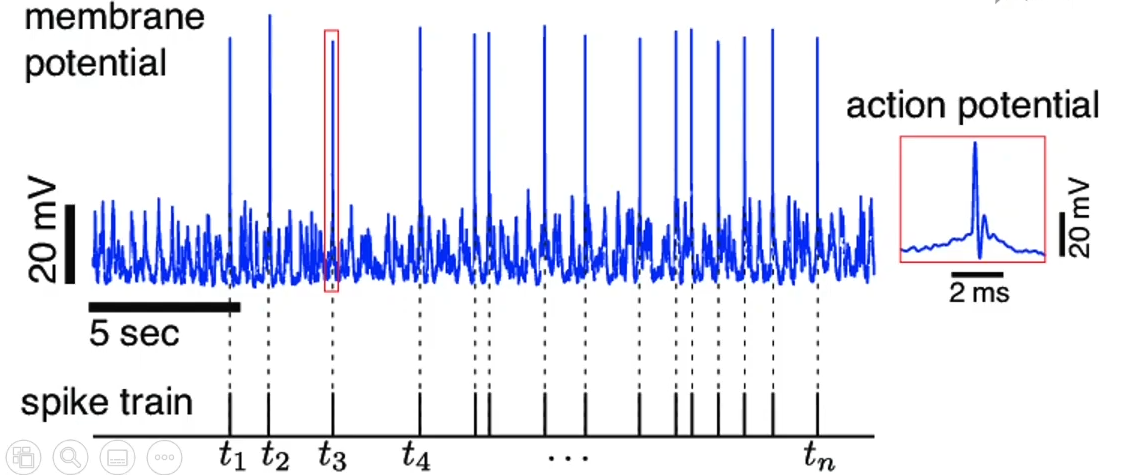
\includegraphics[width=0.6\linewidth]{images/neuronSpikes}
		\caption{Spikes from a noisy signal. Source \cite{dan_goodman_2022_7044500}}
		\label{fig:neuronspikes}
	\end{figure}
	
	\par SNNs possess several noteworthy characteristics that distinguish them from traditional machine learning techniques, including classical neural networks. These distinctions encompass \cite{kasabov2019time}:
	
	\begin{itemize}
		\item Proficiency in modeling temporal, spatial-temporal, or spectro-temporal data.
		\item Effectiveness in capturing processes involving various time scales.
		\item Seamless integration of multiple modalities, such as sound and vision, into a unified system.
		\item Aptitude for predictive modeling and event prediction.
		\item Swift and highly parallel information processing capabilities.
		\item Streamlined information processing.
		\item Scalability, accommodating structures ranging from a few tens to billions of spiking neurons.
		\item Minimal energy consumption when implemented on neuromorphic platforms.
	\end{itemize}
	
	\par In order to emulate such behavior, let's begin with a simple model: The "Leaky Integrate and Fire neuron" (LIF). The LIF model describes the evolution of membrane potential as follows.
	
	\par Here we have the "leaking" equation, which models the potential decay over time.
	\begin{equation}
		\tau \cdot \dfrac{dV}{dt} = -V
		\label{eq:leak}
	\end{equation}
	
	\par When a neuron receives a spike, the membrane potential V increases according to a synaptic weight w.
	\begin{equation}
		V = V + w
	\end{equation}
	
	\begin{figure}
		\centering
		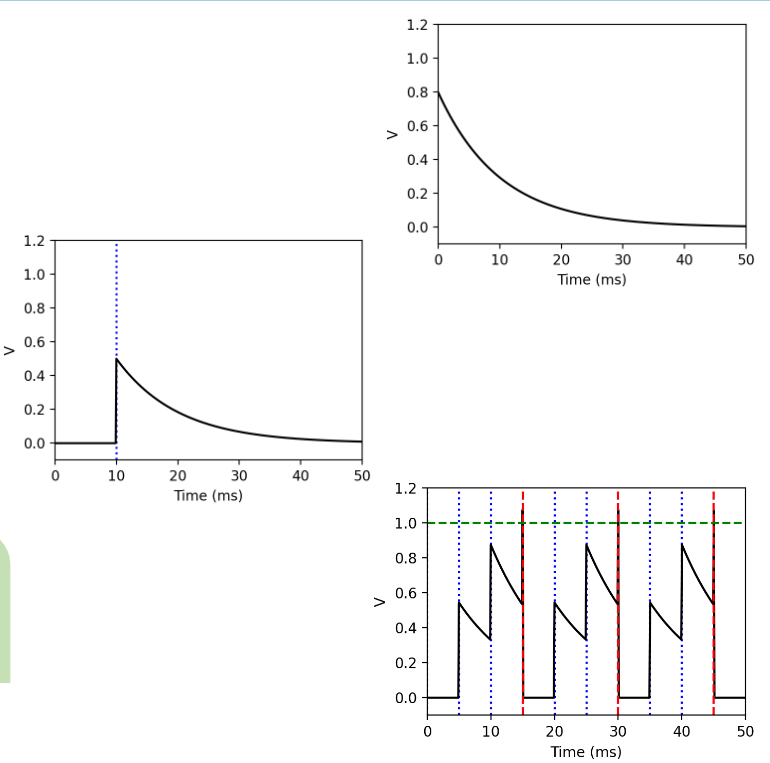
\includegraphics[width=0.5\linewidth]{images/neuronSpikes2}
		\caption{Evolution of a Spike. Source \cite{dan_goodman_2022_7044500}}
		\label{fig:neuronspikes2}
	\end{figure}
	
	\par As shown in Figure \ref{fig:neuronspikes2}, when a neuron reaches a certain threshold, it resets (V = 0) and enters a refractory period.
	
	\par Energy efficiency:
	
	\par Spiking Neural Networks (SNNs) are often considered power-efficient for several reasons:
	
	\begin{enumerate}
		\item Event-Driven Processing: SNNs are inherently event-driven. Instead of constantly updating neuron activations and synapse weights as in traditional artificial neural networks (ANNs), SNNs only transmit spikes (action potentials) when a neuron's membrane potential reaches a certain threshold. This event-driven approach reduces the amount of computation required and can lead to significant energy savings.
		
		\item Sparse Activity: SNNs tend to exhibit sparse activity, meaning that only a small percentage of neurons are active at any given time. This sparsity reduces the number of computations that need to be performed, which is especially beneficial for hardware implementations where most of the energy consumption comes from active components.
		
		\item Low Precision: SNNs can often work with lower precision than ANNs. While ANNs typically use high-precision floating-point numbers for neuron activations and synaptic weights, SNNs can use lower precision fixed-point or binary representations. Lower precision computations require less energy to perform.
		
		\item Neuromorphic Hardware: SNNs can be efficiently implemented on specialized neuromorphic hardware, which is designed to mimic the energy-efficient behavior of biological neural systems. These hardware platforms are optimized for the event-driven nature of SNNs, further reducing power consumption.
		
		\item Energy-Aware Learning Rules: SNNs can employ learning rules that take into account energy efficiency. For example, some learning rules prioritize strengthening or weakening synapses based on their contribution to network activity, which can lead to more energy-efficient learning.
		
		\item Spike Encoding: SNNs can encode information in the timing and frequency of spikes, which can be a highly efficient way to represent and process data, particularly for event-based sensors like vision sensors or auditory sensors.
	\end{enumerate}


	\par How do SNNs get trained? Well, this is still an open question. An SNN neuron has an activation-function behavior that is more relatable to a \textbf{step-function}. Therefore, in principle, we can't use gradient descent-based solutions because this kind of function \textbf{is not} differentiable \cite{kasabov2019time}.
	
	
	\par But there is some insigths out there that may put some light on this subject: While some \textit{in vivo/ in vitro} observations shows that brains in general learns by strengthen/weaken and add/remove synapses or even by creating new neurons or other cumbersome methods like RNA packets. There are some more acceptable ones like \cite{kasabov2019time}:
	
	\begin{itemize}
		\item Spike Timming Dependent Plasticity (STDP): The idea is that if there is a pre-synaptic neuron and it fires \textbf{before} the post-synaptic one there is a strengthening in connection but, if the post-synaptic fire before then we are going to have a weakening .
		\item Surrogate gradient descent: The technique \textbf{approximates} the step-function by using another mathematical function, which is differentiable (like sigmoid), in order train the network. These approximations are used only \textbf{in the backwards pass} keeping the steps function in forward pass \cite{kasabov2019time}.
		\item Evolving algorithms: Uses the selection of the fittest throughout many generations of networks.
		\item Reservoir computing: Echo state networks and Liquid state machines. Which will be discussed further in this presentation.
	\end{itemize} 		
	
	\begin{figure}
		\centering
		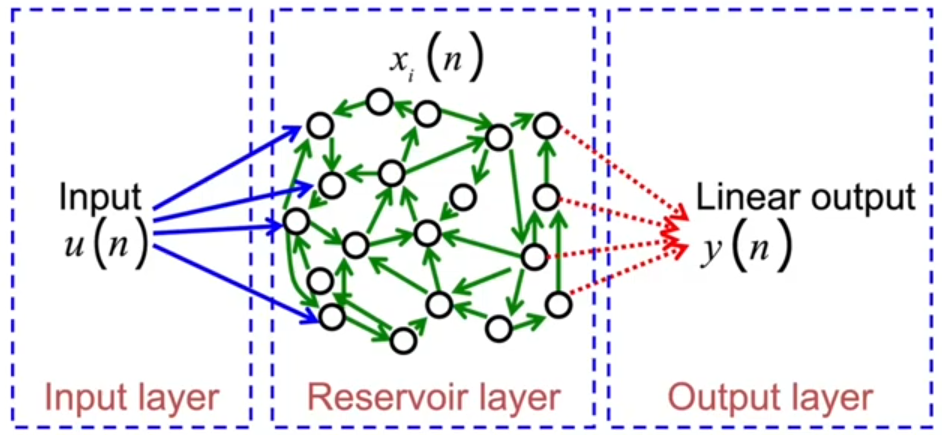
\includegraphics[width=0.7\linewidth]{images/reservoirComputing}
		\caption[Reservoir computing]{Reservoir computing: The reservoir layer is not trained. Intead just the weights between reservoir and output layer are ajusted. Source: \cite{kasabov2019time}}
		\label{fig:reservoircomputing}
	\end{figure}
	



\end{frame}
